%%% LaTeX Template: Two column article
%%%
%%% Source: http://www.howtotex.com/
%%% Feel free to distribute this template, but please keep to referal to http://www.howtotex.com/ here.
%%% Date: February 2011

%%LINHA 37 \usepackage{indentfirst} % parágrafo / indentação
%%LINHA 38 \usepackage{setspace} espaço entre linhas

%%% Preamble
\documentclass[	DIV=calc,%
							paper=a4,%
							fontsize=12pt,%
							onecolumn]{scrartcl}	 					% KOMA-article class

\usepackage{lipsum}													% Package to create dummy text
\usepackage[brazil]{babel}										% English language/hyphenation
\usepackage[protrusion=true,expansion=true]{microtype}				% Better typography
\usepackage{amsmath,amsfonts,amsthm}					% Math packages
\usepackage[pdftex]{graphicx}									% Enable pdflatex
\usepackage[svgnames]{xcolor}									% Enabling colors by their 'svgnames'
\usepackage[hang, small,labelfont=bf,up,textfont=it,up]{caption}	% Custom captions under/above floats
\usepackage{epstopdf}												% Converts .eps to .pdf
\usepackage{subfig}													% Subfigures
\usepackage{booktabs}												% Nicer tables
\usepackage{fix-cm}													% Custom fontsizes
\usepackage[utf8]{inputenc}
\usepackage[top=2.5cm, bottom=2.5cm, left=2.5cm, right=2.5cm]{geometry}
\usepackage[ddmmyyyy]{datetime}
\usepackage{pdfpages}
\addto\captionsenglish{%
	\renewcommand\tablename{Tabela}
	\renewcommand\figurename{Figura}
} 
 

 
%%% Custom sectioning (sectsty package)
\usepackage{sectsty}													% Custom sectioning (see below)
\usepackage{indentfirst} % parágrafo / indentação
\usepackage{setspace}

\allsectionsfont{%															% Change font of al section commands
	\usefont{OT1}{phv}{b}{n}%										% bch-b-n: CharterBT-Bold font
	}

\sectionfont{%																% Change font of \section command
	\usefont{OT1}{phv}{b}{n}%										% bch-b-n: CharterBT-Bold font
	}



%%% Headers and footers
\usepackage{fancyhdr}												% Needed to define custom headers/footers
	\pagestyle{fancy}														% Enabling the custom headers/footers
\usepackage{lastpage}	

% Header (empty)
\lhead{}
\chead{}
\rhead{}
% Footer (you may change this to your own needs)

%% ====================================
%% ====================================
%% mude o rodape  do projeto
%% ====================================
%% ====================================

\lfoot{\footnotesize \texttt{Cabeamento estruturado} \textbullet ~Instituto Ambiental do Paraná}


\cfoot{}
\rfoot{\footnotesize página \thepage\ de \pageref{LastPage}}	% "Page 1 of 2"
\renewcommand{\headrulewidth}{0.0pt}
\renewcommand{\footrulewidth}{0.4pt}



%%% Creating an initial of the very first character of the content
\usepackage{lettrine}
\newcommand{\initial}[1]{%
     \lettrine[lines=3,lhang=0.3,nindent=0em]{
     				\color{DarkGoldenrod}
     				{\textsf{#1}}}{}}



%%% Title, author and date metadata
\usepackage{titling}															% For custom titles

\newcommand{\HorRule}{\color{DarkGoldenrod}%			% Creating a horizontal rule
									  	\rule{\linewidth}{1pt}%
										}

\pretitle{\vspace{-30pt} \begin{flushleft} \HorRule 
				\fontsize{50}{50} \usefont{OT1}{phv}{b}{n} \color{DarkRed} \selectfont 
				}

%% ====================================
%% ====================================
%% mude o titulo  do projeto
%% ====================================
%% ====================================

\title{Projeto de cabeamento estruturado na Infraestrutura de Rede do Instituto Ambiental do Paraná}					% Title of your article goes here

%% ====================================



\posttitle{\par\end{flushleft}\vskip 0.5em}

\preauthor{\begin{flushleft}
					\large \lineskip 0.5em \usefont{OT1}{phv}{b}{sl} \color{DarkRed}}
\author{André Luis Finatto, Diogo Witt, Jedielson de Souza, Paulo Cesar Cardoso de Campos}  	% Author name goes here


\postauthor{\footnotesize \usefont{OT1}{phv}{m}{sl} \color{Black} 
					\\Universidade Tecnológica Federal do Paraná - Câmpus Cornélio Procópio 								% Institution of author
					\par\end{flushleft}\HorRule}

\date{}																				% No date




%%% Begin document
\begin{document}
\maketitle
\thispagestyle{fancy} 	
\thispagestyle{empty}		% Enabling the custom headers/footers for the first page 
% The first character should be within \initial{}




%% ====================================
%% ====================================
%% mude o resumo  do projeto
%% ====================================
%% ====================================

\initial{O}\textbf{presente projeto visa apresentar uma reestruturação fictícia na infraestrutura baseada no ambiente real do Instituto Ambiental do Paraná. O Projeto aborda o levantamento da planta física, elaboração da planta lógica e equipamentos passivos da rede.}


%% ====================================
\begin{figure}
	\centering
	
\includegraphics{utfpr}
\end{figure}

\vspace{2cm}
\centerline{\textit{\textbf{\today}}}

\clearpage
    \renewcommand*\listfigurename{Lista de figuras}
\listoffigures

\renewcommand*\listtablename{Lista de tabelas}
\listoftables




\clearpage
\renewcommand{\contentsname}{Sumário}
\tableofcontents
\clearpage

%% ====================================
%% ====================================
%% Inicio do texto
%% ====================================
%% ====================================
\section{Introdução}
\onehalfspacing % espaçamento 1,5 entre linhas
Este projeto tem como propósito levantar os requisitos e propor soluções no âmbito da rede de computadores do Instituto Ambiental do Paraná – IAPAR (unidade de Curitiba),  vinculado à Secretaria da Agricultura e do Abastecimento (SEAB) do Estado do Paraná, constituindo-se no órgão de pesquisa que dá embasamento tecnológico as políticas públicas de desenvolvimento rural do Estado do Paraná.
O ambiente do Instituto Ambiental do Paraná é formado por técnicos responsáveis por trabalhos e rotinas administrativas, além de emissão de licenças e análises ambientais.
Atualmente são utilizados 33 desktops, além de 27 ramais telefônicos, 2 impressoras e uma central telefônica.
O objetivo do presente projeto é definir requisitos, materiais e planos de execução para conectar os vários elementos computacionais, com intuito de se utilizar de maneira compartilhada e eficiente todos seus recursos disponíveis. 
Assim sendo, o presente projeto constitui-se no primeiro item de documentação da rede a ser implantada.

\subsection{Benefícios}
Após a execução do projeto, a infraestrutura de redes e dados estará mais segura, proverá maior desempenho e estará menos suscetível a intercorrências que possam vir a causar sua paralisação. O suporte será mais simples e rápido, além de facilitar em possíveis mudanças de posições de equipamentos.

\subsection{Organizações Envolvidas}
%Coloque o nome de todas as organizações envolvidas. Se for um projeto real, identifique quais as responsabilidades de cada uma das organizações. É comum que em um projeto de redes (cabeamento), temos várias organizações, sendo que cada uma delas com uma determinada responsabilidade.
%Sugestão: crie uma tabela contento a relação delas.
\begin{table}[h!] % coloque h! para forcar a posicao
\onehalfspacing
\centering
\caption{Atividades e respectivos responsáveis}
\vspace{0.5cm}
\label{tab1}
\resizebox{\textwidth}{!}{%
	\begin{tabular}{|c|c|}
		\hline
		\textbf{Responsabilidade}                                           & \textbf{Organização}            \\ \hline
		Serviços de Internet 1                                              & Empresa Provedora de Internet 1 \\ \hline
		Serviços de Internet 2 – (Redundância)                              & Empresa Provedora de Internet 1 \\ \hline
		Levantamento de Requisitos                                          & Grupo                           \\ \hline
		Desenvolvimento do Projeto                                          & Grupo                           \\ \hline
		Orçamento dos ativos e passivos de rede                             & Grupo                           \\ \hline
		Aquisição dos ativos e passivos de rede                             & Setor Compras - Contratante     \\ \hline
		Instalação de eletrocalhas                                          & Contratante                     \\ \hline
		Instalações elétricas adequadas (tomadas, aterramento, para-raios)  & Contratante                     \\ \hline
		Instalação dos pontos de rede Ethernet (descritos na planta lógica) & Grupo                           \\ \hline
		Passagem do cabeamento (horizontal e backbone)                      & Grupo                           \\ \hline
		Instalação e configuração de todos ativos e passivos de rede        & Grupo                           \\ \hline
	\end{tabular}%
}

\end{table}

\section{Estado atual}
%Aprente o estado atual da rede. Caso não tenha rede, desconsiderar esta seção.

%Caso tenha rede, deixe claro:
%\begin{itemize}
%	\item os passivos de rede atuais:path panels, cabos, etc..;
%	\item as principais reclamações dos usuários. Qual o principal motivo da reestruturação? Efetue uma pesquisa junto aos colaboradores para determinar quais problemas a rede apresenta.
%	\item Observações. Analise a rede e verifique se há estruturas que não se enquadram nas normas ou que indicam suspeita de problemas.
%\end{itemize}

\section{Requisitos}
\begin{itemize}
\item Rede escalável;
\item VLANs delimitando departamentos, bem como o tráfego de dados e voz;
\item Largura de banda capaz de atender demandas como: compartilhamentos de arquivos entre usuários, videoconferências, acesso remoto;
\item Servidor de arquivos;
\item Servidor de impressões;
\item Permitir que usuários de outras unidades possam se autenticar na rede local quando em trânsito;
\item Permitir que usuários;
\item Acesso e gerenciamento seguro de banco de dados;
\item Promover mecanismos que garanta a segurança da rede local;
\item Permitir o desenvolvimento e manutenção de serviços WEB, para permitir o acesso interno e externo às páginas e sistemas;
\item Analisar, avaliar, definir e adotar processos, técnicas e ferramentas para o desenvolvimento de software;
\item Administrar a infraestrutura de rede, diagnosticar problemas com seus componentes ou com o comportamento de computadores ligados à ela;
\item Instalação, configuração e manutenção dos sistemas computacionais (hardware e Software) da sede e das unidades descentralizadas, bem como prover treinamento, diagnosticar e resolver problemas inerentes aos sistemas computacionais.
\end{itemize}

\section{Usuários e Aplicativos}
O prédio é formado por dois andares. No térreo estão a Recepção, Licenciamento Florestal, Fiscalização, Arquivo e Combustível. No primeiro andar estão a Chefia, Arquivo, Licenciamento Industrial, Administrativo e Escritório Regional.\par
Por se tratar de um órgão público, ele depende de editais de seleção para aumento de seu quadro funcional, fato que não costuma ser constante.\par
Porém, devido a também possuir um caráter de instituto de pesquisa, atuando na área educacional, oferecendo curso de pós graduação stricto sensu (Mestrado em agricultura conservacionista), todo ano recebe cerca de 20 alunos novos.\par
Outro fator que pode refletir no aumento de usuários, são as contratações de consultores externos, mas que também são incluídos como usuários da rede.

\subsection{Usuários}
%Crie uma relação da quantidade, perfil de usuários de seu projeto.
\begin{table}[h!] % coloque h! para forcar a posicao
\onehalfspacing
\caption{Usuários e Aplicativos}
\vspace{0.5cm}
\centering
\label{tab2}
\resizebox{\textwidth}{!}{%
\begin{tabular}{|c|c|}
\hline
\textbf{Usuários}        & \textbf{Aplicativos}                                                 \\ \hline
Diretor                  & Microsoft Office, Videoconferência, Aplicações Web,                  \\ \hline
Recepcionista            & Microsoft Office, Controle de Acesso, Aplicações Web,                \\ \hline
Técnicos Administrativos & Microsoft Office, Videoconferência                                   \\ \hline
Pesquisadores            & Microsoft Office, Aplicações Web, Softwares de Análises Estatísticas \\ \hline
Alunos do Mestrado       & Microsoft Office, Aplicações Web, Softwares de Análises Estatísticas \\ \hline
\end{tabular}%
}

\end{table}

%\subsection{Aplicativos}
%Crie uma relação dos aplicativos e seus níveis críticos de uso.

\section{Estrutura predial existente}

%Explique aqui a planta física dos prédios
%Pode ser anexada, em escala ou não.

%Deve conter uma descrição geral, indicando a possível distância entre os pontos de rede e restrições de instalação.
\begin{figure}[h!]
	\centering
	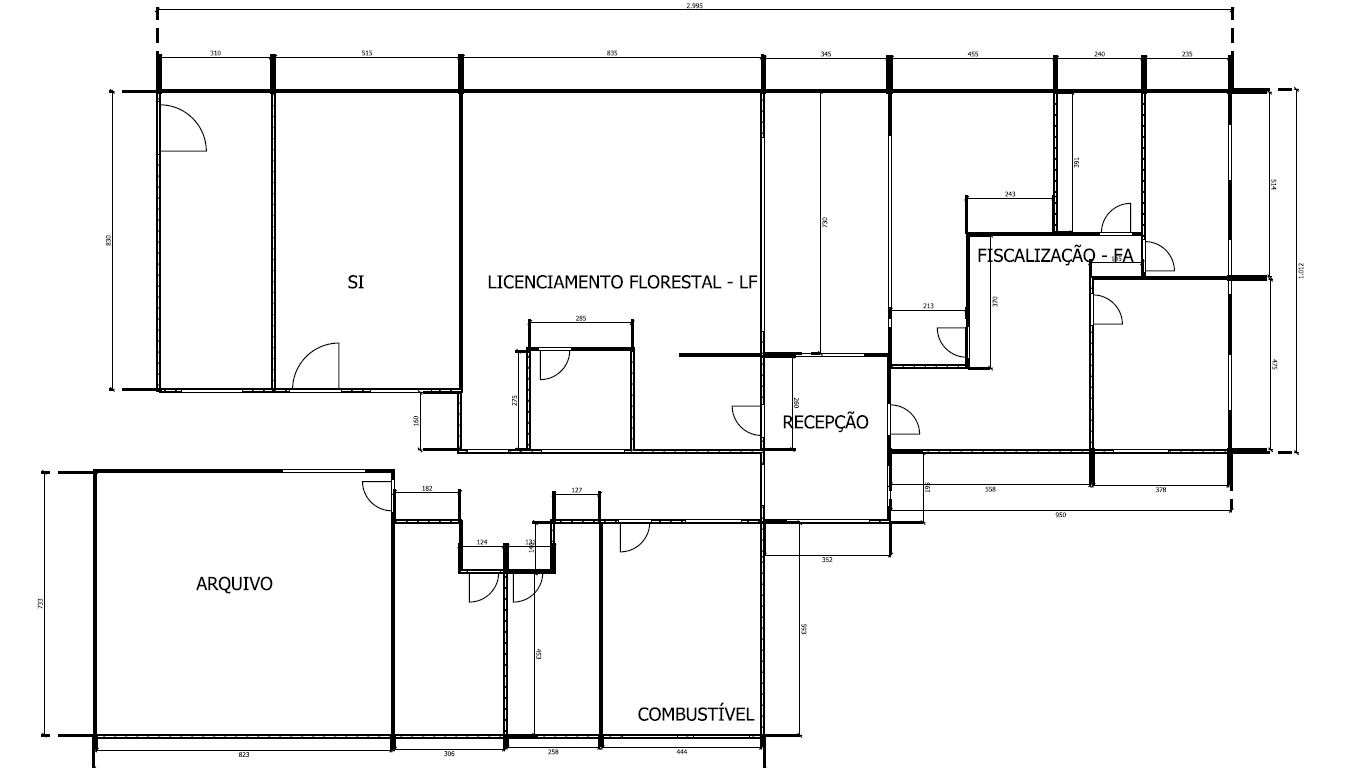
\includegraphics[width=\textwidth]{figura1.png}
	\caption[Planta Baixa Térreo]{Planta Baixa Térreo}
	\label{fig:figura1}
\end{figure}

\begin{figure}[h!]
	\centering
	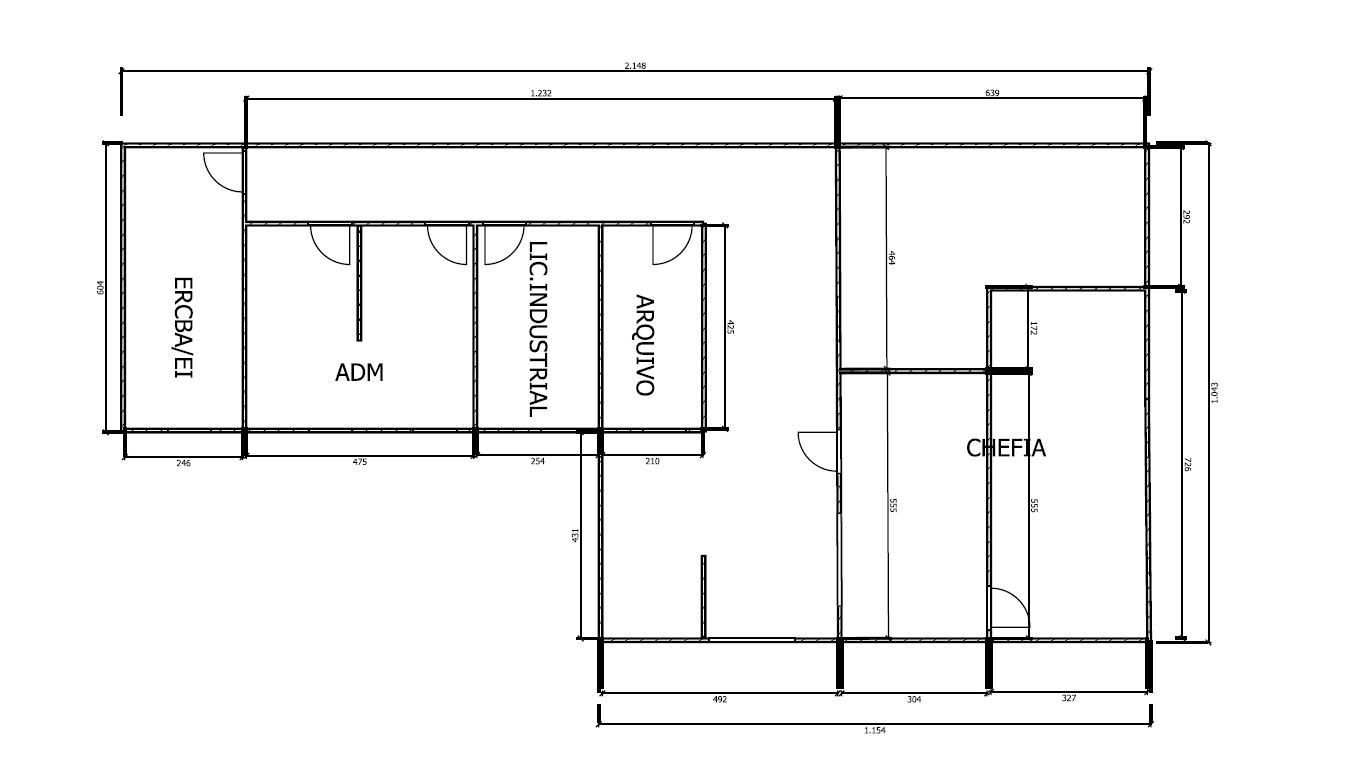
\includegraphics[width=\textwidth]{figura2.png}
	\caption[Planta baixa 1º andar IAPAR]{Planta baixa 1º andar IAPAR}
	\label{fig:figura2}
\end{figure}

\section{Planta Lógica - Elementos estruturados}

\subsection{Estado atual}
%Deve ter a planta atual, se for o caso
\begin{figure}[h!]
	\centering
	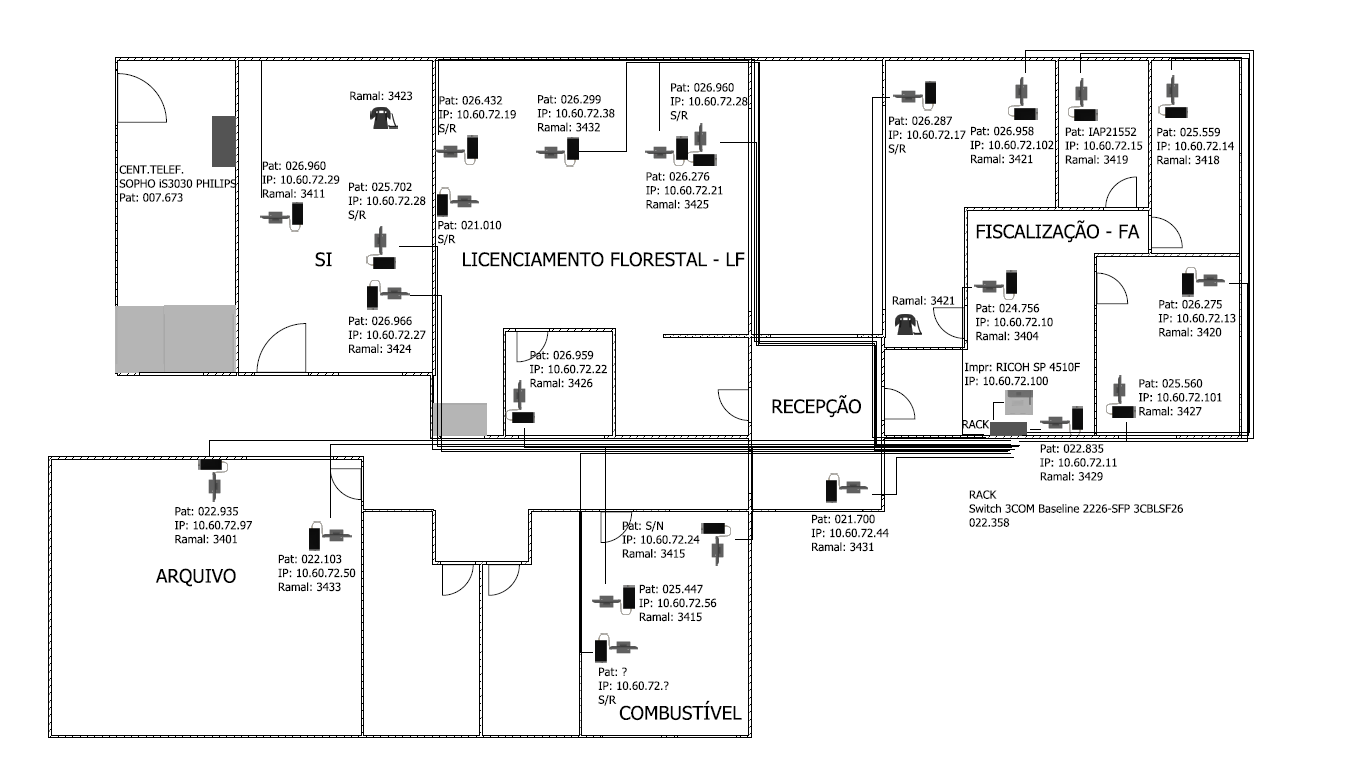
\includegraphics[width=\textwidth]{figura3.png}
	\caption[Estado Atual - Posições das Áreas de Trabalho - Térreo]{Estado Atual - Posições das Áreas de Trabalho - Térreo}
	\label{fig:figura3}
\end{figure}

\begin{figure}[h!]
	\centering
	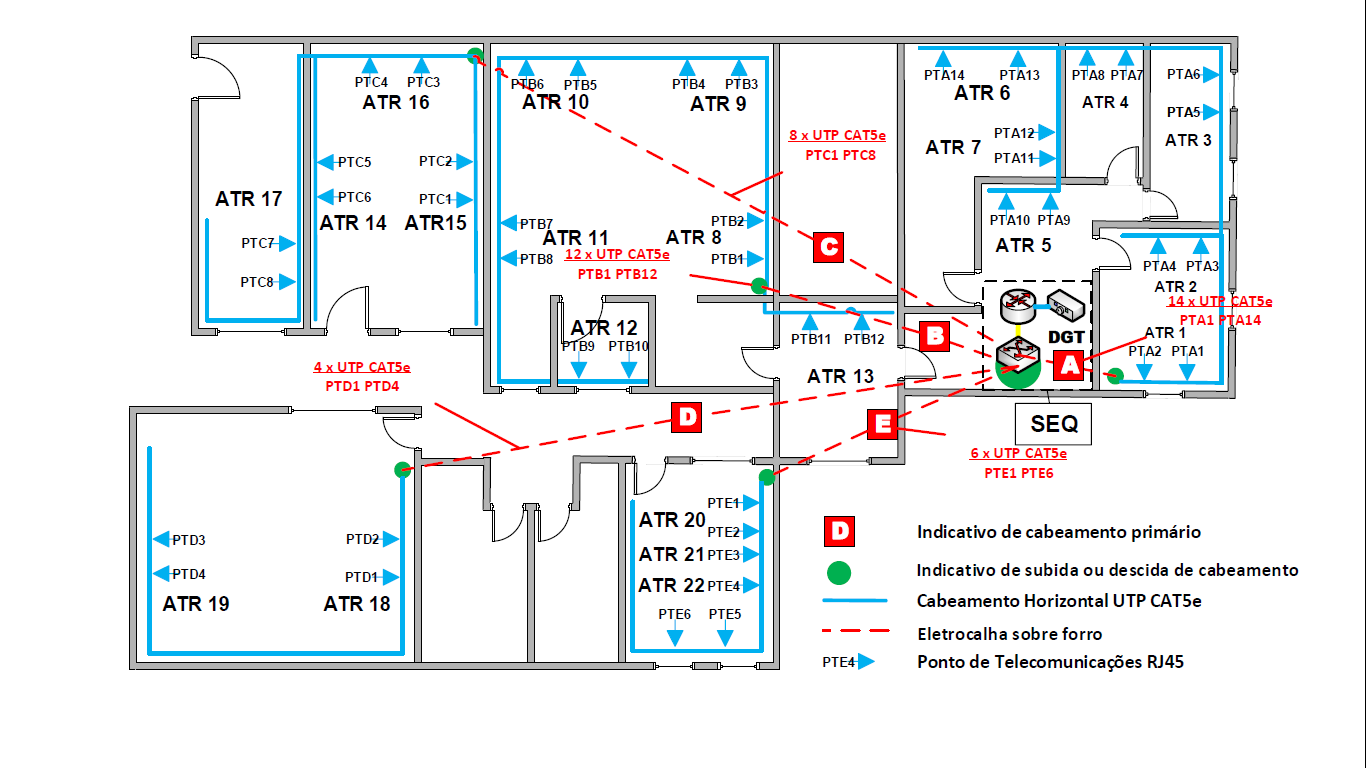
\includegraphics[width=\textwidth]{figura4.png}
	\caption[Estado Atual - Distribuição Cabeamento Horizontal/Backbone - Térreo]{Estado Atual - Distribuição Cabeamento Horizontal/Backbone - Térreo}
	\label{fig:figura4}
\end{figure}

\begin{figure}[h!]
	\centering
	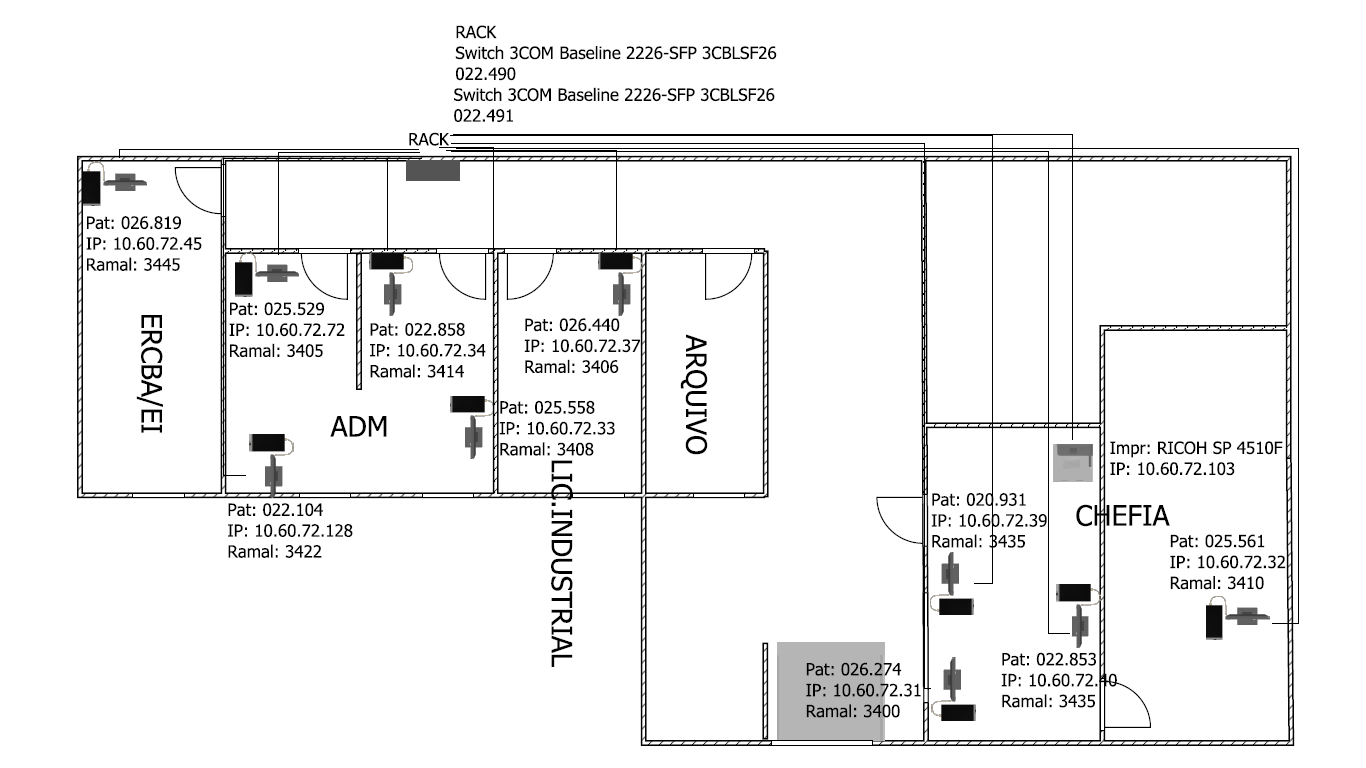
\includegraphics[width=\textwidth]{figura5.png}
	\caption[Trabalho - Térreo]{Estado Atual - Posições das Áreas de Trabalho - Térreo}
	\label{fig:figura5}
\end{figure}

\begin{figure}[h!]
	\centering
	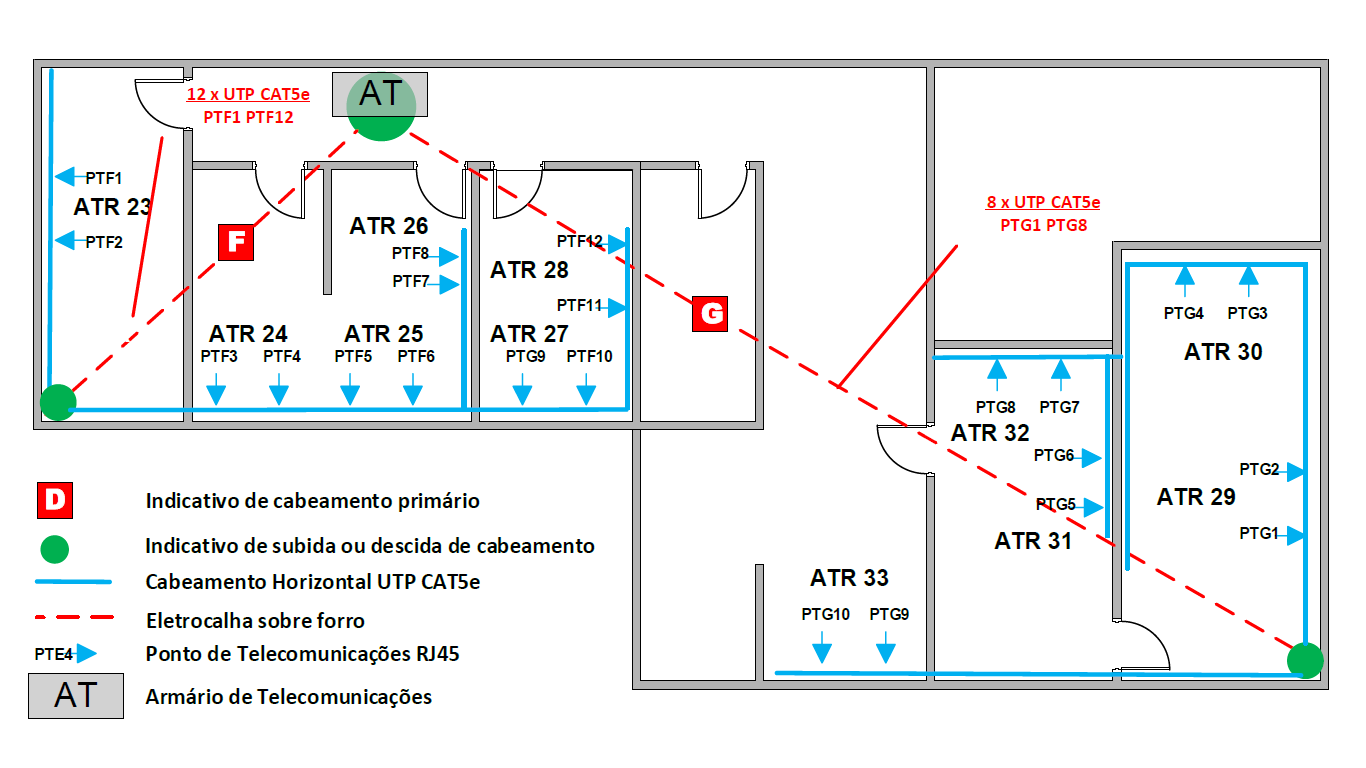
\includegraphics[width=\textwidth]{figura6.png}
	\caption[Estado Atual - Distribuição Cabeamento Horizontal/Backbone – 1º andar]{Estado Atual - Distribuição Cabeamento Horizontal/Backbone – 1º andar}
	\label{fig:figura6}
\end{figure}

\subsection{Topologia}
%Proposta futura, proposta após implantação.
%Deve conter o diagrama da rede. Atente-se a redundância  e ligações truncadas.
%Deve explicar todos termos e componentes utilizados nestas plantas. Por exemplo: entrance facility, work area, horizontal cabling, etc..

%Todos os elementos das figuras devem ser explicados. 
%Crie esboço da configuração dos racks e brackets. Explique cada um dos componentes. Você pode criar uma tabela contendo figuras dentro, ou criar uma tabela e incluí-la como imagem. Por exemplo, verifique a tabela \ref{tab1}.

%\begin{table}[h!] % coloque h! para forcar a posicao
\onehalfspacing
\centering
\caption{Atividades e respectivos responsáveis}
\vspace{0.5cm}
\label{tab1}
\resizebox{\textwidth}{!}{%
	\begin{tabular}{|c|c|}
		\hline
		\textbf{Responsabilidade}                                           & \textbf{Organização}            \\ \hline
		Serviços de Internet 1                                              & Empresa Provedora de Internet 1 \\ \hline
		Serviços de Internet 2 – (Redundância)                              & Empresa Provedora de Internet 1 \\ \hline
		Levantamento de Requisitos                                          & Grupo                           \\ \hline
		Desenvolvimento do Projeto                                          & Grupo                           \\ \hline
		Orçamento dos ativos e passivos de rede                             & Grupo                           \\ \hline
		Aquisição dos ativos e passivos de rede                             & Setor Compras - Contratante     \\ \hline
		Instalação de eletrocalhas                                          & Contratante                     \\ \hline
		Instalações elétricas adequadas (tomadas, aterramento, para-raios)  & Contratante                     \\ \hline
		Instalação dos pontos de rede Ethernet (descritos na planta lógica) & Grupo                           \\ \hline
		Passagem do cabeamento (horizontal e backbone)                      & Grupo                           \\ \hline
		Instalação e configuração de todos ativos e passivos de rede        & Grupo                           \\ \hline
	\end{tabular}%
}

\end{table}
\begin{figure}[h!]
	\centering
	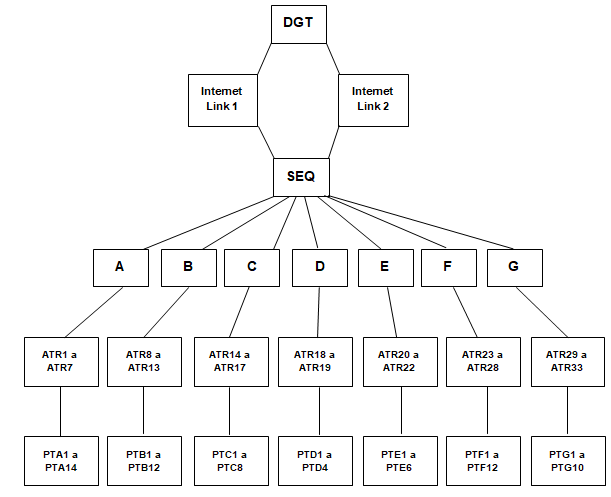
\includegraphics[width=\textwidth]{figura7.png}
	\caption[Diagrama da Topologia da Rede]{Diagrama da Topologia da Rede}
	\label{fig:figura7}
\end{figure}

\subsection{Encaminhamento}
%Eletrodutos, calhas, e qualquer material em que os cabos serão alojados/alocados.

\subsection{Memorial descritivo}

%Relacione todos os equipamentos passivos que serão utilizados, tipo, fabricante, quantidade.

\subsection{Identificação dos cabos}
%Explique como os cabos serão identificados em seu projeto. Coloque uma relação dos cabos instalados e identificados.

\section{Implantação}
%Estabeleça um cronograma de implantação:
%Remoção de equipamentos existentes (destino para descarte), instalação dos condutores, instalação dos cabos, 
%identificação dos cabos, montagem dos racks, certificação, etc... Crie atividades e estabeleça o tempo de execução. Se for um projeto real, indique também quais os responsáveis pela execução do projeto e de cada uma das etapas.

%Defina marcas (e padrões) e fornecedores se for o caso. Atenção a contratados e subcontratados para a realização das atividades. Estabeleça a responsabilidade de execução da atividade e também da validação dela.

%Utilize algum software para gerear o cronograma. Excel,etc. O fundamental é dividir em etapas, descrever e estimar o tempo de cada uma delas.

%Segue uma relação de ferramentas:
%http://asana.com/, \\
%https://trello.com/, \\
%http://www.ganttproject.biz/, \\
%http://www.orangescrum.org/. 

\section{Plano de certificação}
A certificação da planta se dará após completo o processo de implantação e antes do início de operação da rede. Toda a estrutura de rede passará pelo processo de certificação.\\
Será agendada uma data e hora com o IAP-PR, para que também possam acompanhar a atividade.\\
No processo serão realizados os seguintes testes:
\begin{itemize}
\item Wiremap - Teste que verifica a continuidade dos fios;
\item WireLenght - Teste que verifica o comprimento dos cabos;
\item Resistance Test - Teste que verifica a resistência do circuito em cada fio;
\item NEXT/FEXT - Teste que identifica possíveis falhas nos conectores e ruídos gerados por dispositivos externos;
\item Atenuação - Teste que identifica falha de atenuação no cabo;
\item Perda de Retorno - Teste que mede a reflexão no cabo;
\item Impedância - Teste que calcula a impedância do cabo;
\item Testes Delay e Skew - Teste que mede o tempo que um sinal leva para percorrer o cabo e a diferença entre o maior e menor tempo medidos;
\item Capacitância - Teste que mede a capacitância mútua entre os dois condutores de cada par;
\item ACR e Power Sum ACR - Teste que realiza faz a subtração entre os resultados de atenuação e o teste NEXT, em um par (ACR) ou nos outros três pares do cabo (Sum ACR).
\end{itemize}
\par Os testes serão realizados a fim de alcançar a certificação Cat5E.
Caso algum teste não obtenha os resultados esperados, será identificado o cabo ou cabos com problema para que sejam efetuadas as correções necessárias para o alcançe da certificação.
Após o fim do processo, será entregue um relatório ao IAP-PR contendo todos os resultados obtidos nos testes acima mencionados.

\section{Plano de manutenção}
A instalação possui 1 ano de garantia contra defeitos em cabeamento e conectores. Não está incluso o serviço de mudança de pontos e certificações de novos pontos. É possível ao IAP, dentro do período de garantia, solicitar até 3 (três) manutenções preventivas, a fim de identificar e prevenir a ocorrência de falhas na rede.
Como se trata de órgão público, a posterior contratação de empresa para manutenção, mudança ou criação de novos pontos dependerá de novo processo licitatório

%Revisões periódicas na rede, emissão de certificados para novos pontos.

\subsection{Plano de expansão}
%Existe um plano de expansão? Quantos novos pontos poderão ser acrecidos na rede, antes de migração de equipamentos na camada 2? Se houver expansão, quais equipamentos deverão ser direcionados para as estremidades da rede? 
Não há plano de expansão para a rede, uma vez que a infraestrutura predial não suporta mais estações de trabalho devido a limitações físicas.\par
Porém em caso de necessidade de ampliação, a margem é ínfima pois sobrarão poucos recursos de rede sem utilização. No térreo estão previstos 44 pontos de comunicação RJ45, além do cascateamento entre os 2 switches do térreo e o cabeamento vertical para o switch do primeiro andar, totalizando 47 portas em uso. Ainda há a abordagem do provedor de telecomunicações, que caso ocorra em mídia elétrica consumirá a última interface RJ45 disponível dos switches. Caso essa abordagem seja óptica utilizando a interface SFP do equipamento, sobrará uma interface RJ45 no térreo.\par
Já no primeiro andar, estão previstos 22 pontos de comunicação RJ45.  Somados ao cabeamento vertical, utilizarão 23 interfaces elétricas de um total de 24 disponíveis no switch.\par
Portanto tanto no térreo quanto no primeiro andar não há margem para ampliação sem a aquisição de novos materiais, como switches e patch pannels com maior densidade de interfaces, além da criação de novos pontos de telecomunicações e cabeamento.

\section{Risco}
%Enumerar e explicar os riscos do projeto.
O objetivo do projeto de cabeamento estruturado é mitigar todas as etapas e diminuir a probabilidade de riscos inerentes ao projeto. Porém mesmo com todos os cuidados ainda há riscos que devemos considerar:
\begin{itemize}
\item Como a compra dos materiais utilizados se dará pela internet e de lojas de outras cidades, há o risco de atraso na entrega ou entrega de material diferente do pedido, o que gerará atraso no cronograma do projeto.

\item Devido ao fato do prédio não ser novo, há a possibilidade de encontrar passagens obstruídas, além de dificuldade na passagem das canaletas.

\item Outra questão de infraestrutura a ser considerada é a rede elétrica existente. Falhas e instabilidades nessa área podem provocar instabilidades na rede de dados em geral.

\item Outro risco que apesar de poder ser minimizado com treinamento e supervisão dos responsáveis pela instalação é a falha humana durante a execução das atividades. Estas possíveis falhar serão identificadas durante a certificação e poderão ser corrigidas, porém provocarão atraso na entrega da obra. 

\item Por fim nosso cenário atual mostra que ainda existem riscos externos que não são mensuráveis e podem ocorrer sem responsabilidade de nenhum dos entes do projeto. Como exemplo podemos citar a pandemia do novo Coronavírus que afetaria de sobremaneira o andamento do projeto.
\end{itemize}

\section{Orçamento}
%Crie uma relação de orçamentos baseado na seções anteriores.

\section{Recomendações}
%Observações e recomendações para o cliente.
\clearpage
\section{Referências bibliográficas}
%Utilize o mendley, o jabref ou diretamente o bibtex para gerenciar suas referências biliográficas. As referências são criadas automaticamente de acordo com o uso no texto.

%Exemplo: Redes de computadores, segundo \cite{t2013} é considerada..... Já \cite{kurose2010} apresenta uma versão...

%Analisando os pressupostos de \cite{ref3} e \cite{ref4} concluimos que....


\renewcommand\refname{} %%Referências bibliográficas}  
\bibliographystyle{ieeetr}
\bibliography{referencias}  

%% ***********************************************************************
%% === remover daqui =====================================================
%% ***********************************************************************
=================================================
%%\section{Elementos textuais - Alguns exemplos}

%%Esta seção apresenta exemplos de elementos textuais. \textbf{Remova-a da versão final do texto}.


%%\subsection{Colocar elementos em itens}

%%Texto antes da lista

%%\begin{itemize}
%%	\item First item in a list 
%%	\item Second item in a list 
%%	\item Third item in a list
%%\end{itemize}

%%\subsubsection{Uma subseção de terceiro nivel}

%%Exemplo de uma subseção Tabela \ref{tab1}

%%\subsection{Tabelas}

%%Utilize o site http://www.tablesgenerator.com/ para elaborar as tabelas de seu trabalho.
%%Para adicionar uma tabela utilize: a tag input, passando o arquivo da tabela como parametro
%%\begin{table}[h!]
	\onehalfspacing
	\caption{Tabela Explicativa dos Elementos Constituintes da Rede}
	\vspace{0.5cm}
	\centering
	\renewcommand{\arraystretch}{1.4}
	\label{tab3}
	\resizebox{\textwidth}{!}{%
	\begin{tabular}{|l|l|}
		\hline
		\multicolumn{1}{|c|}{\textbf{Elemento}} & \multicolumn{1}{c|}{{\color[HTML]{000000} \textbf{Função}}}                                                                                                                                                                                                        \\ \hline
		DGT                                     & {\color[HTML]{000000} Distribuidor Geral de Telecomunicações}                                                                                                                                                                                                      \\ \hline
		{\color[HTML]{000000} SEQ}              & {\color[HTML]{000000} Sala de Equipamentos}                                                                                                                                                                                                                        \\ \hline
		A, B, C, D, E, F, G                     & {\color[HTML]{000000} Cabeamento Horizontal Sobre Forro}                                                                                                                                                                                                           \\ \hline
		ART                                     & {\color[HTML]{000000} \begin{tabular}[c]{@{}l@{}}Cabeamento Horizontal Baixo, encaminhado via calhas de rodapé, os \\ quais atendem cada uma das áreas de trabalho. Sua identificação é composta \\ por: ART+”Nº da área de trabalho correspondente”\end{tabular}} \\ \hline
		PTXN                                    & {\color[HTML]{000000} \begin{tabular}[c]{@{}l@{}}Pontos de Rede RJ45 com sua devida identificação, composta pelo padrão: \\ PT+”Letra do Cabeamento Horizontal Sobre Forro”+”Nº do Ponto”\end{tabular}}                                                            \\ \hline
	\end{tabular}
}
\end{table}

%%Dentro do arquivo você deve definir o label e pode utilizá-lo para referenciar. Exemplo:
%%Na tab \ref{tab2} temos a relação de ....


%%Você também pode modificar a tabela manualmente, incluindo, por exemplo h! dentro de sua definição. Veja no exemplo tab2.tex

%%\subsection{Figuras}

%%As figuras podem ser no formato PDF, JPG, PNG. Você pode referenciá-las da mesma maneira que tabelas. Exemplo: A figura \ref{fig1} apresenta.....

%%Não se preocupe o local em que a figura será renderizada em seu texto. Preocupe-se em criar referência para ela, ou seja, toda figura e tabela deve conter pelo menos uma referência no texto.

%%\begin{figure}
%%\centering
%%\includegraphics[width=\textwidth]{fig1}
%%\caption{Exemplo de figura com escala horizontal}
%%\label{fig1}
%%\end{figure}


%%\begin{figure}
%%	\centering
%%	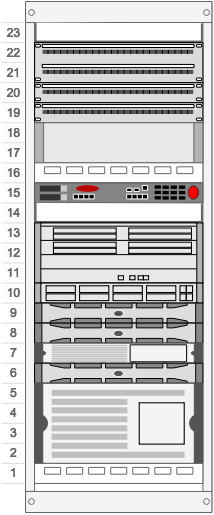
\includegraphics[]{fig2}
%%	\caption{Exemplo de figura sem escala}
%%	\label{fig2}
%%\end{figure}

%%Você pode rotacionar figuras também. Para isso utilize o parâmetro angle=-90. Repare que a escala da figura foi modificada pelo parametro height. Você também pode utilizar scale

%%\begin{figure}
%%	\centering
%%	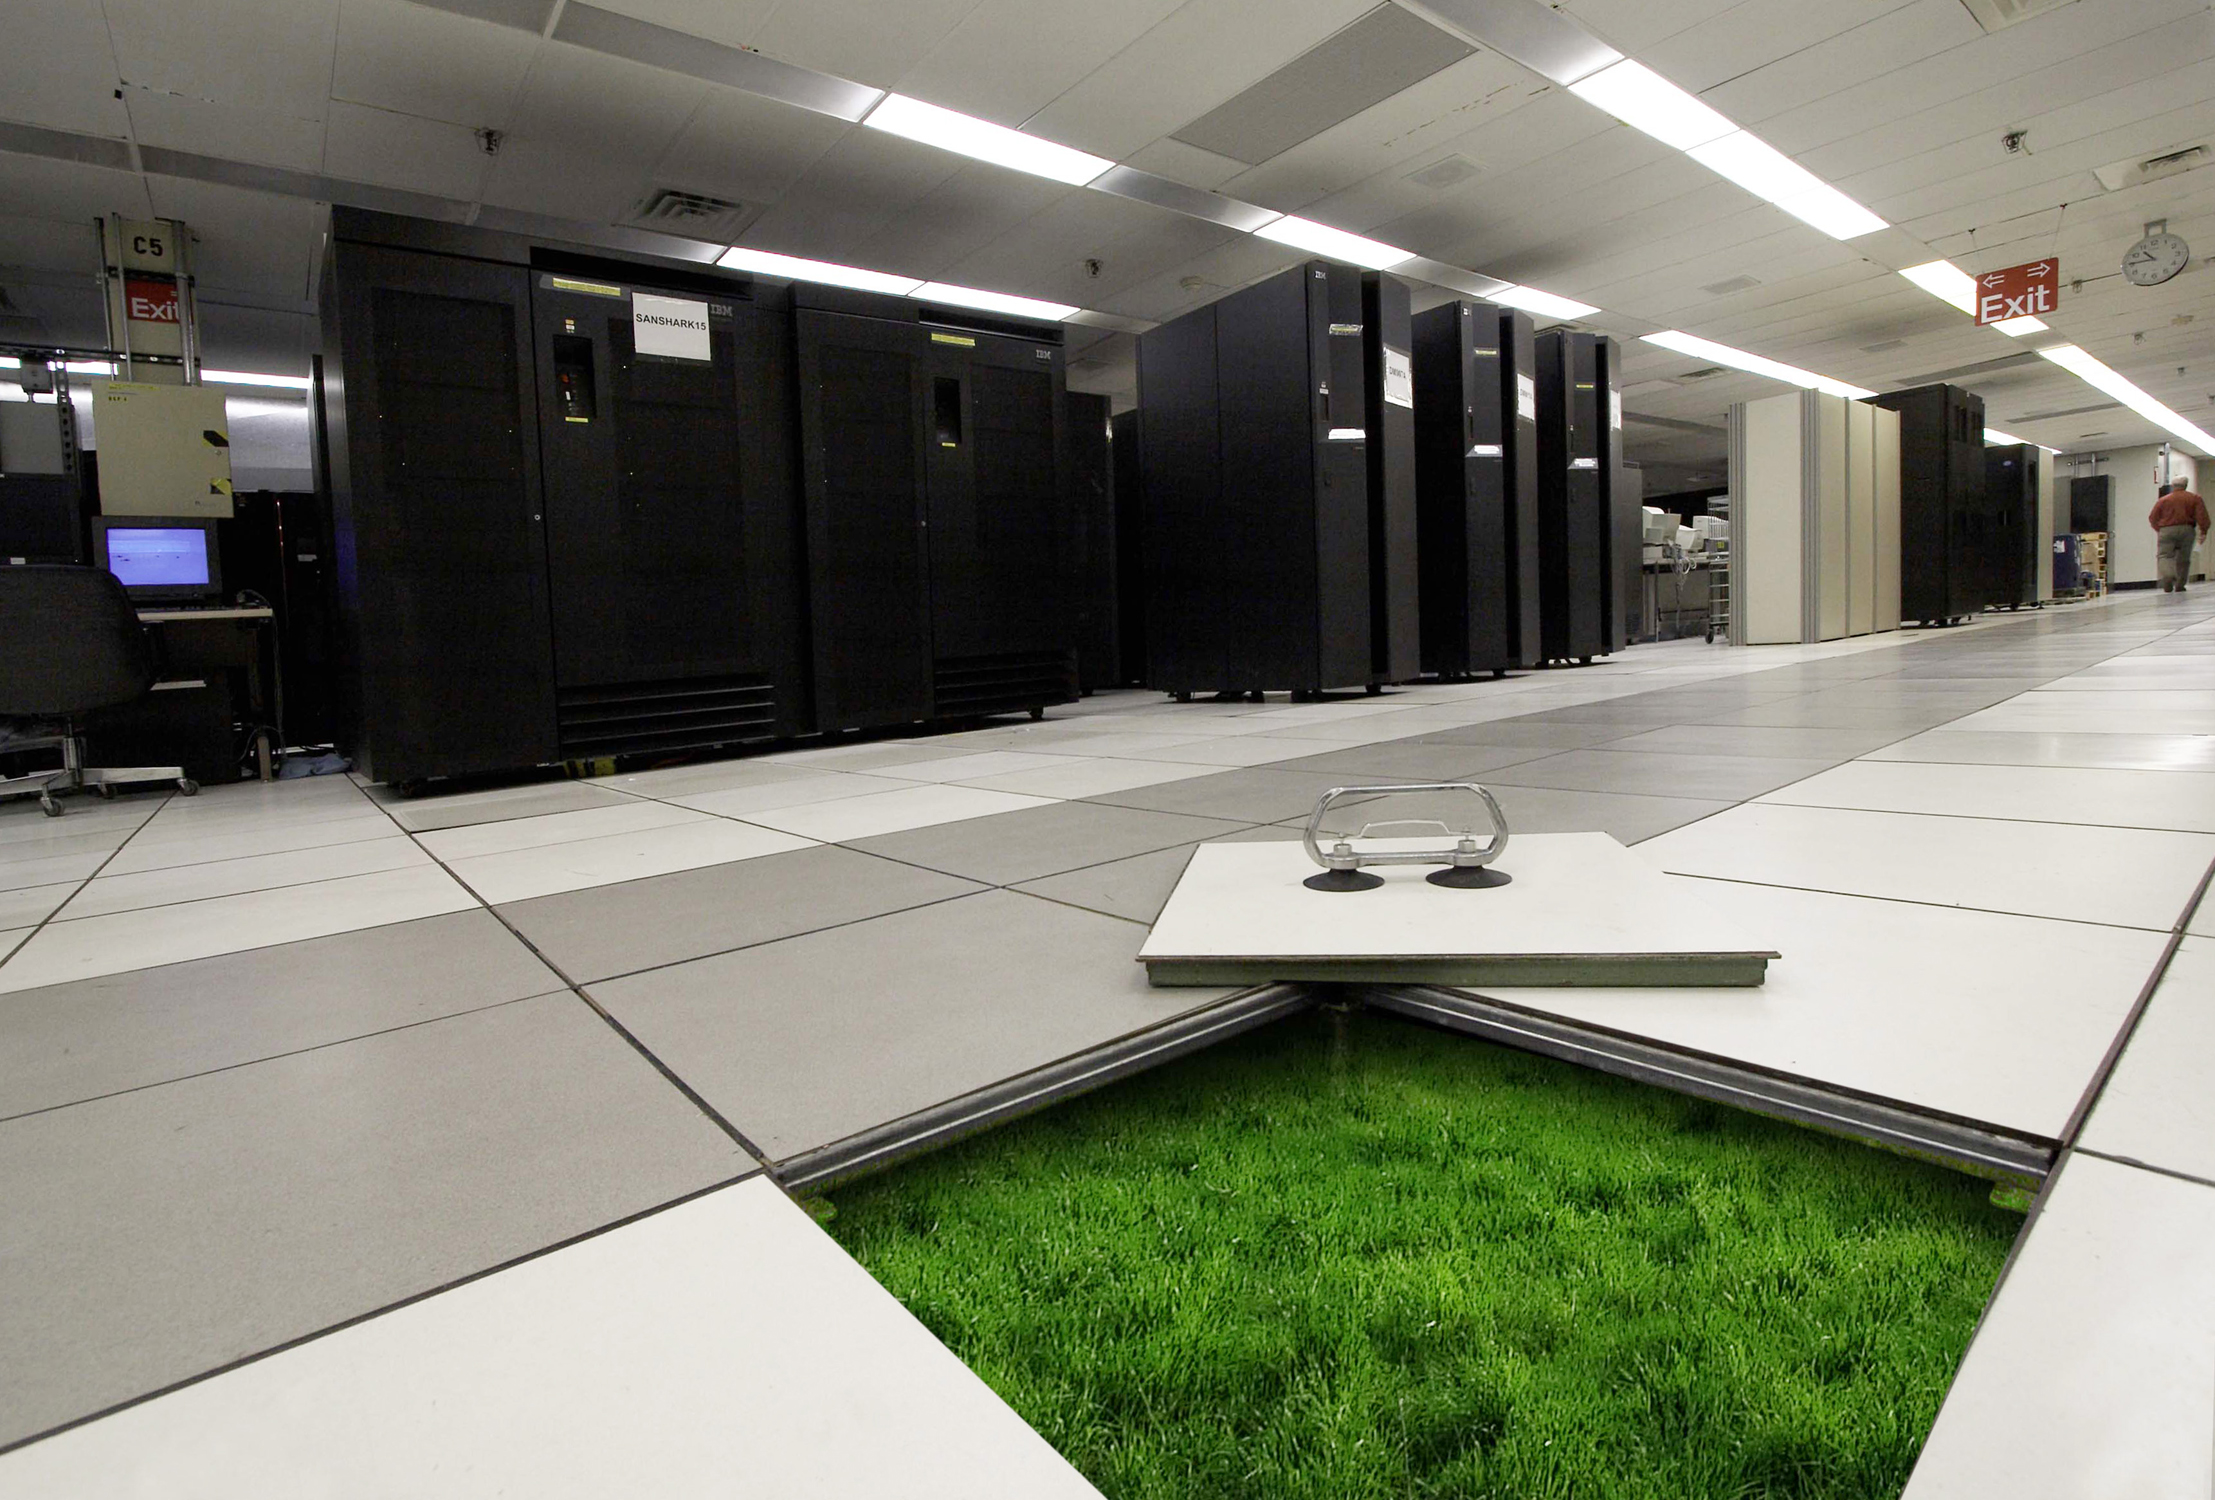
\includegraphics[height=\textwidth,angle=-90]{fig3}
%%	\caption{Exemplo de figura rotacionada}
%%	\label{fig3}
%%\end{figure}

%%Você também pode inserir páginas de outro tamanho em seu texto. Isto irá ajudar a inserir imagens maiores, como as desenvolvidas em CAD. Segue um exemplo na figura \ref{fig4} e figura \ref{fig5}.


%inicio dos comandos para criar uma nova pagina A3
%%\clearpage
%%\KOMAoptions{paper=a3, pagesize}
%%\recalctypearea

%%\begin{figure}
%%	\centering
%%	\makebox[\textwidth][c]{
%%		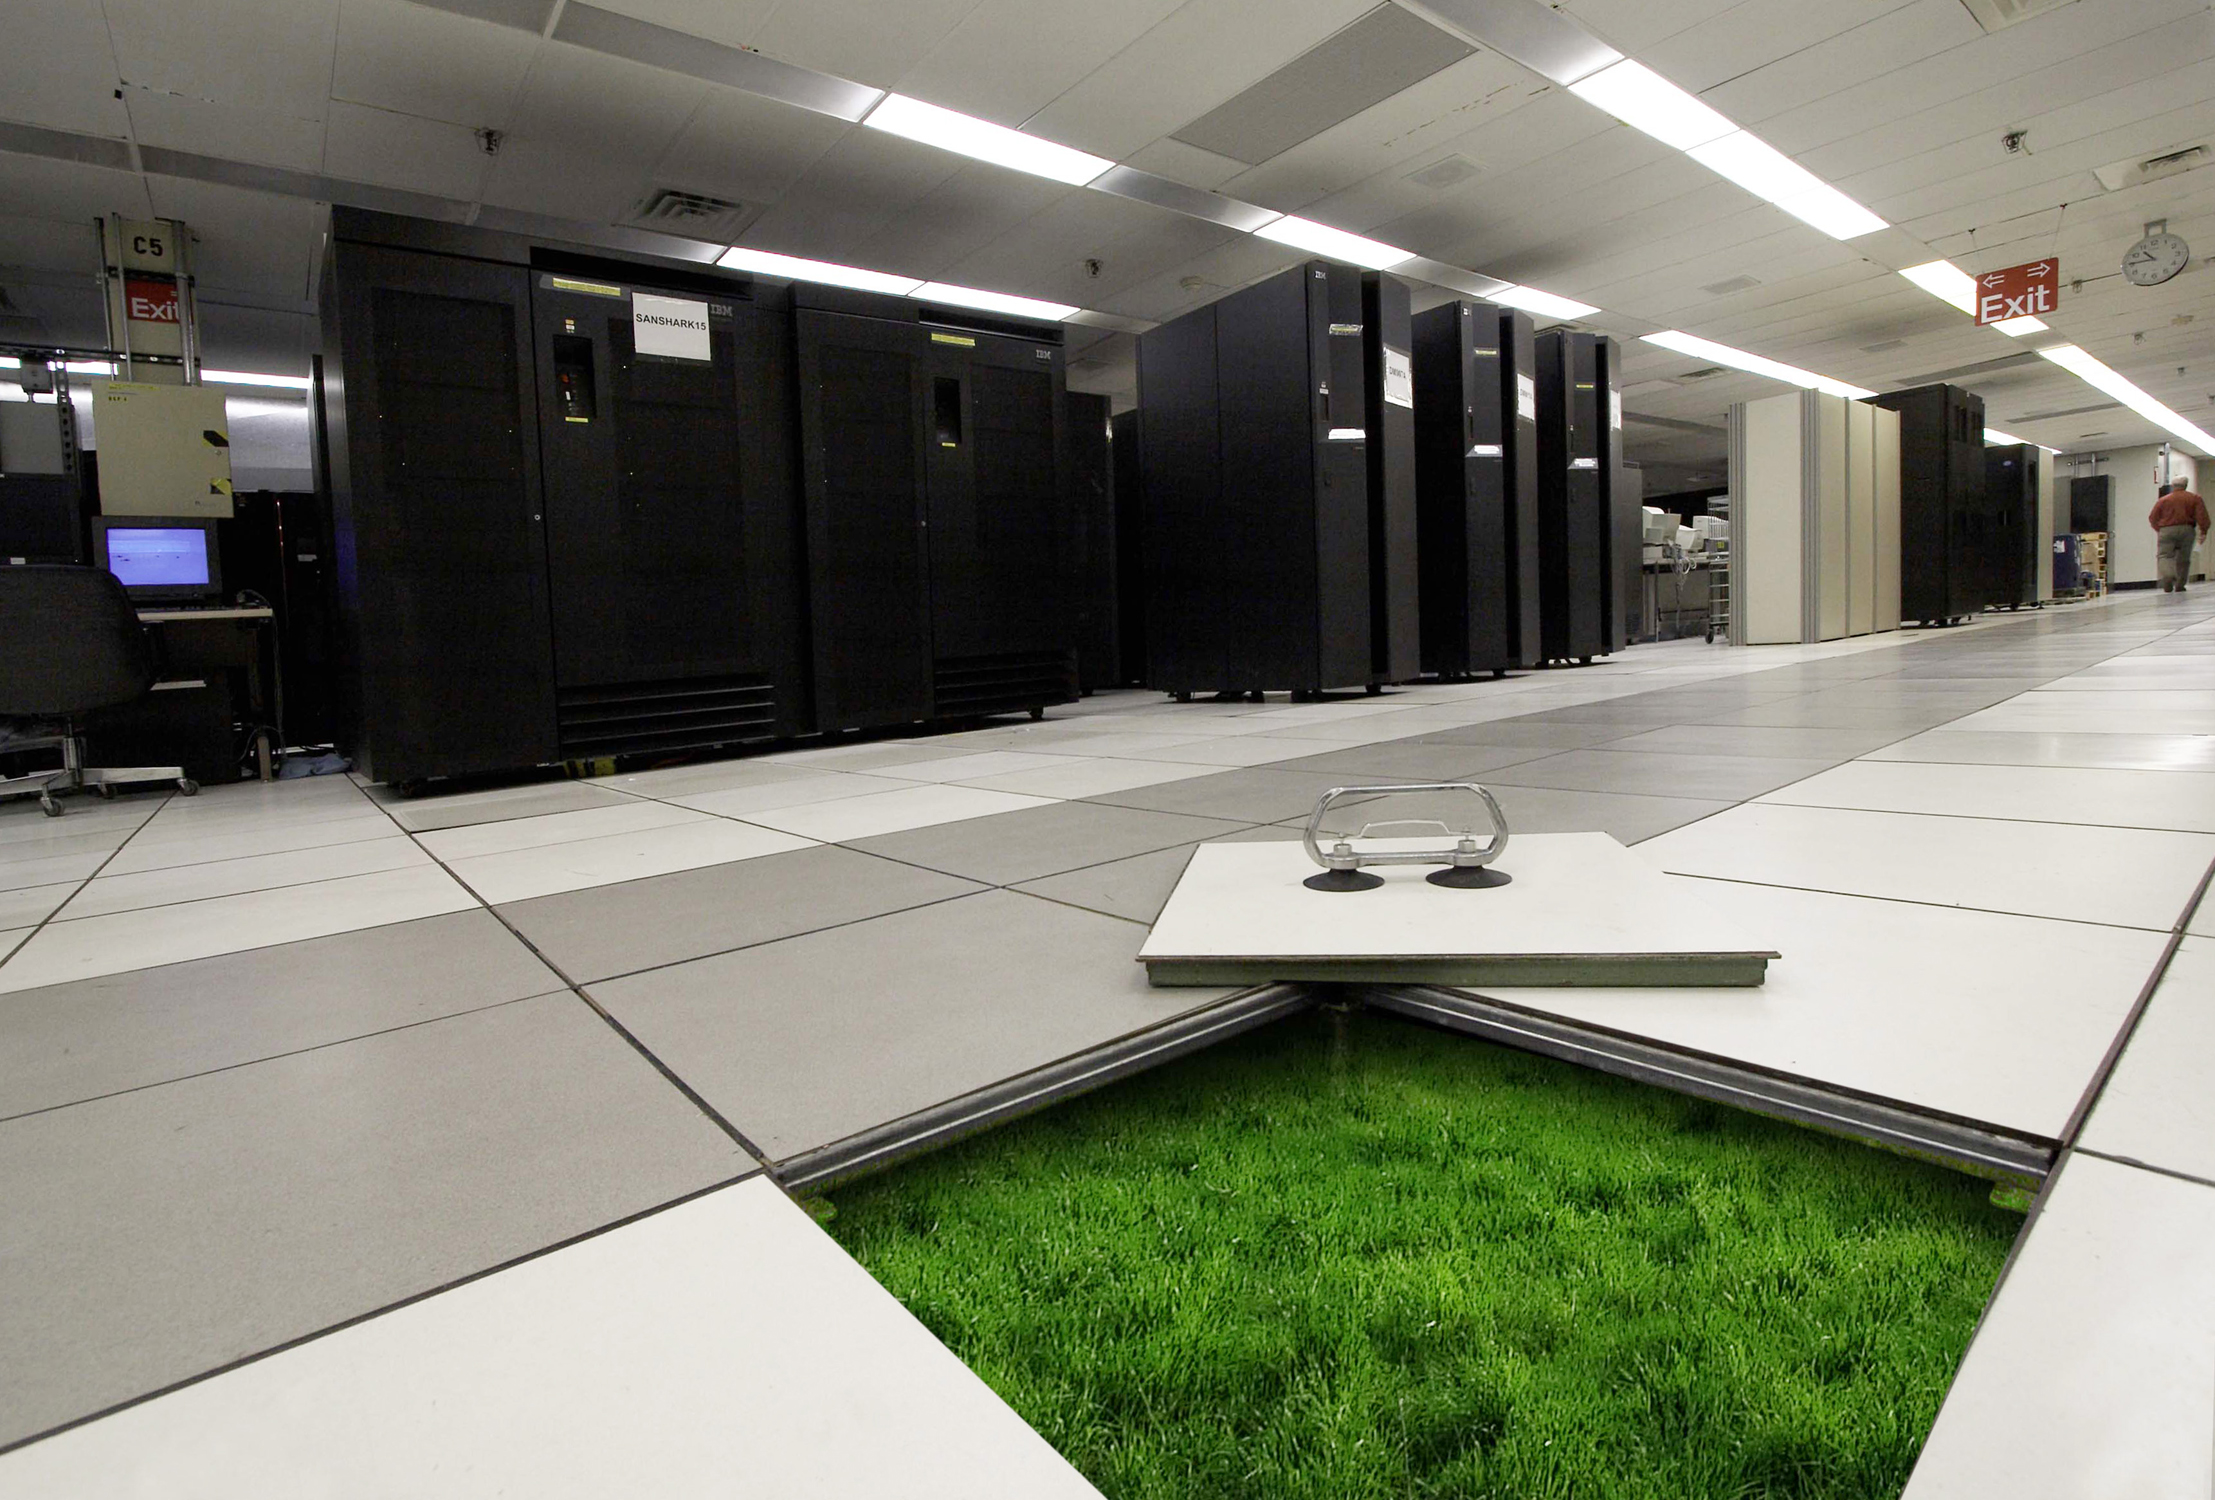
\includegraphics[height=\textheight]{fig3}}
%%	\caption{Exemplo de figura inserida em uma página A3}
%%	\label{fig4}
%%\end{figure}

%Retornar ao formato A4
%%\clearpage
%%\KOMAoptions{paper=a4, pagesize}
%%\recalctypearea
%-- reinicio em A4 


%inicio dos comandos para criar uma nova pagina A3 horizontal
%%\clearpage
%%\KOMAoptions{paper=a3, paper=landscape, DIV=20}
%%\recalctypearea

	
%%\begin{figure}
%%	\centering
%%	\noindent\makebox[\textwidth][c]{
%%		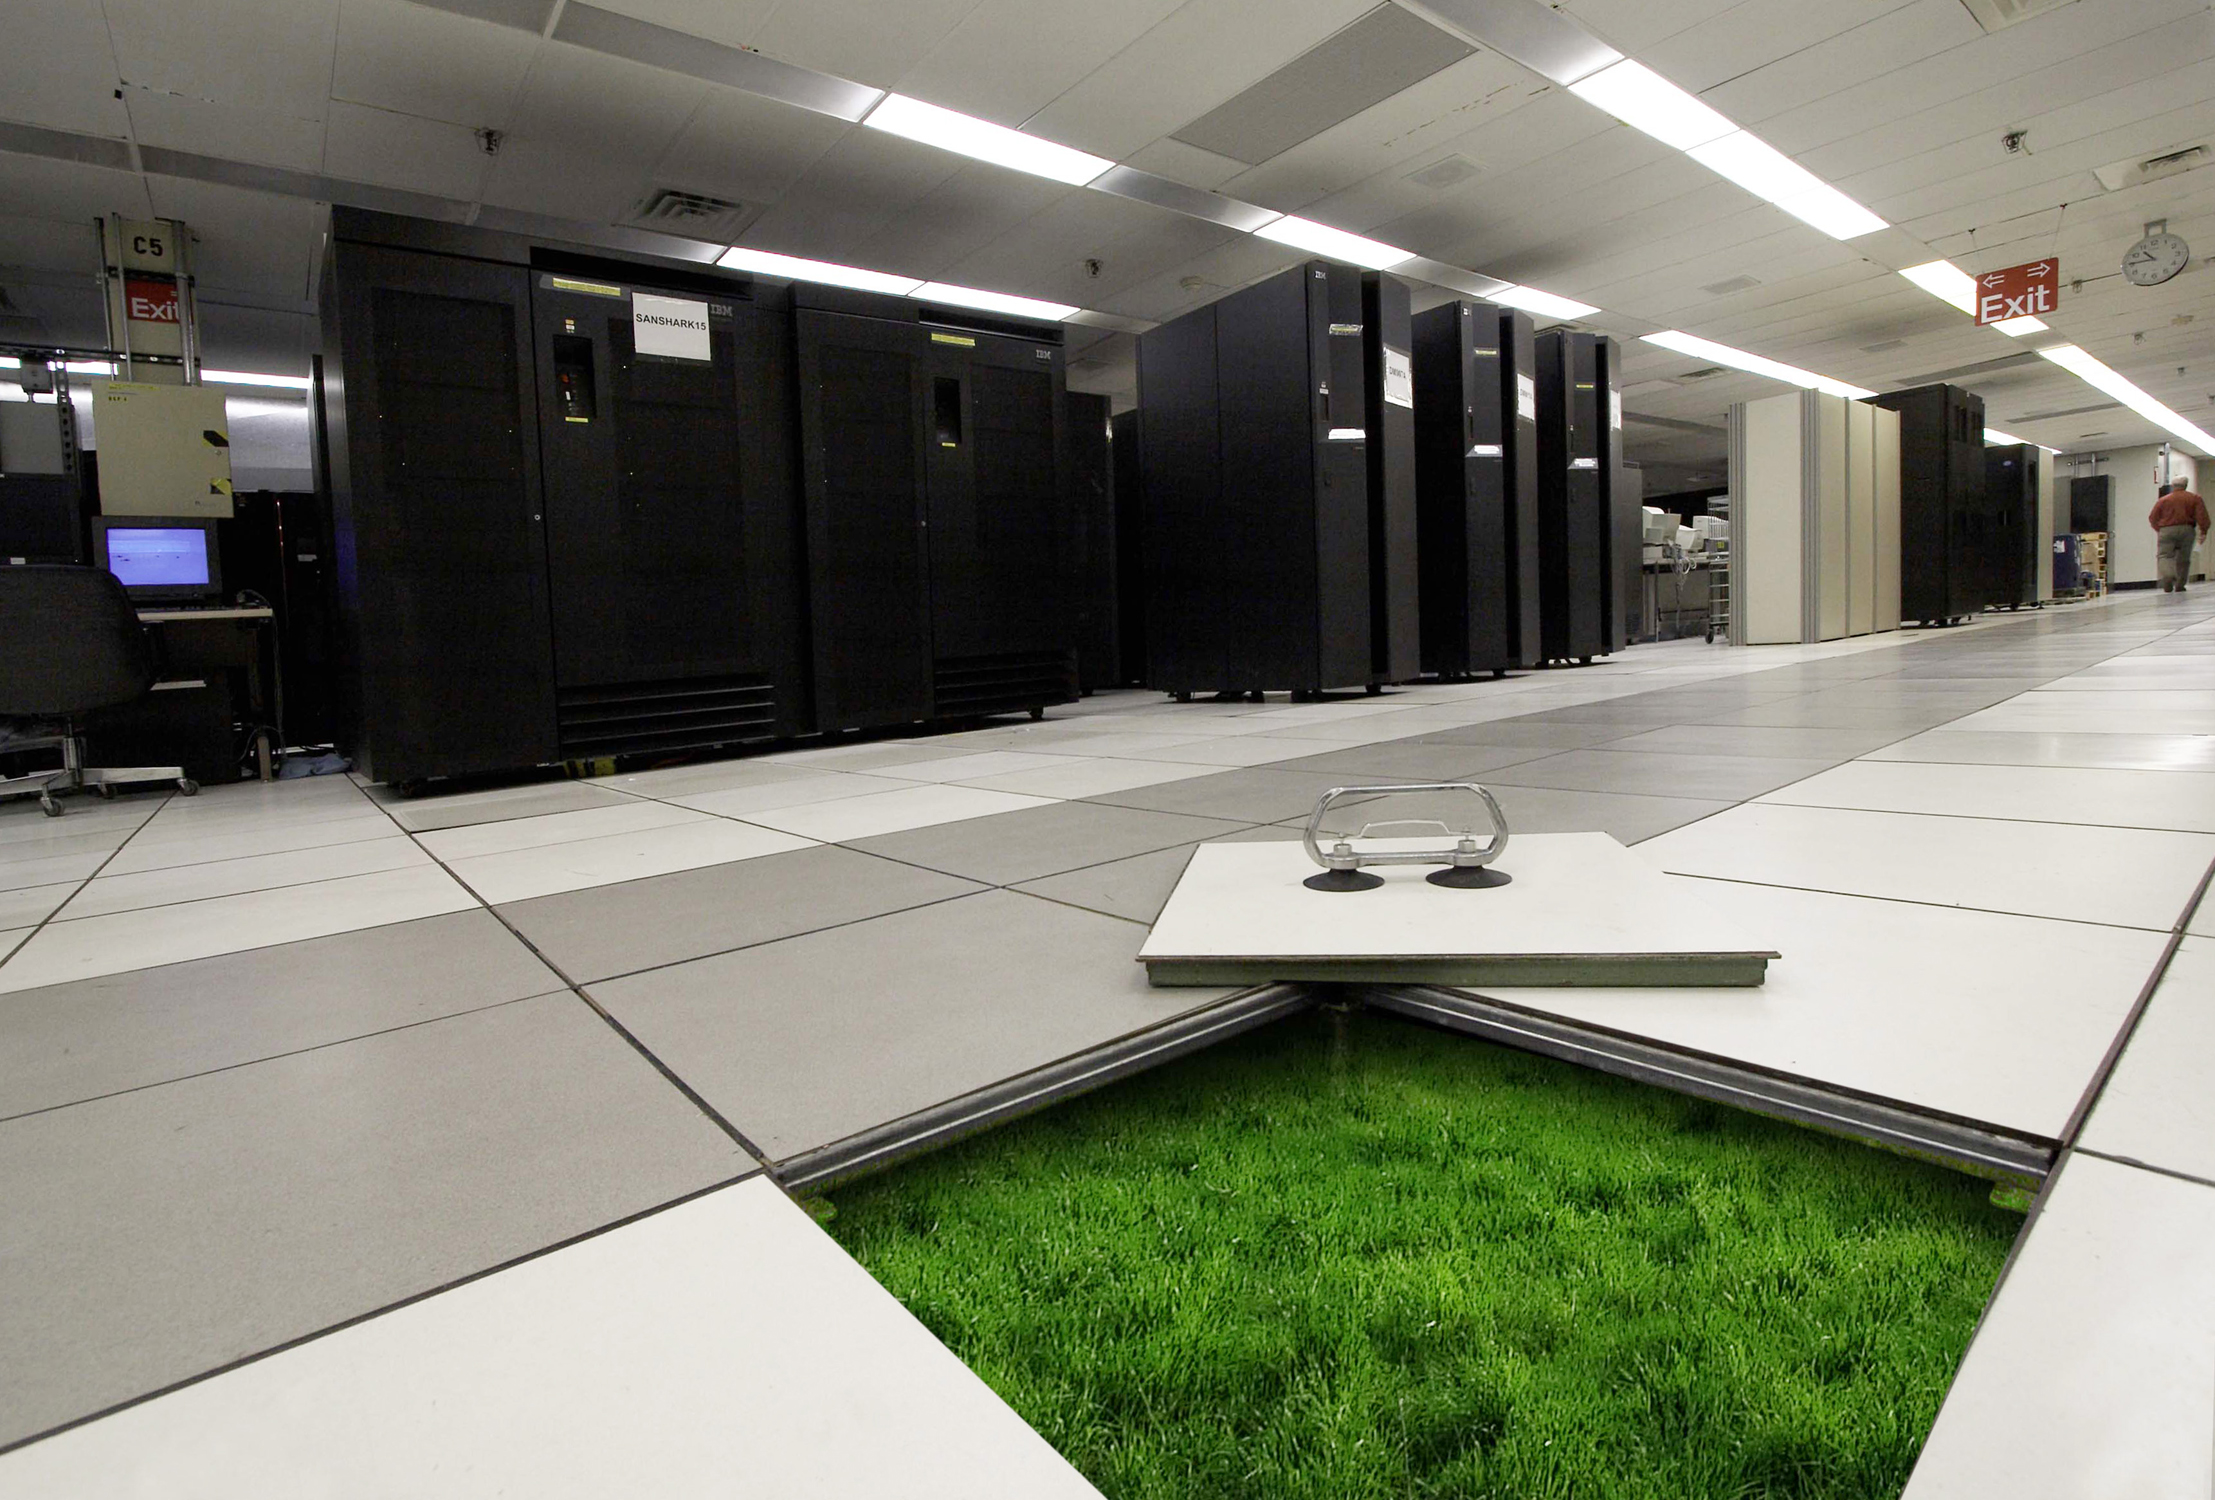
\includegraphics[width=\textwidth]{fig3}
%%	}
%%	\caption{Exemplo de figura inserida em uma página A3 no formato horizontal}
%%	\label{fig5}
%%\end{figure}

%Retornar ao formato A4
%%\clearpage
%%\KOMAoptions{paper=a4, paper=portrait, DIV=15}
%%\recalctypearea
%-- reinicio em A4 


%%\subsubsection{Resumo gráfico}

%%Você pode optar por fazer um resumo no formato de mapa mental/conceitual. 
%%Aqui foi utilizado o site https://app.mindmup.com para gerar o mapa.

%%Para utilizar o resumo gráfico, remova o texto da seção resumo (linha 137) e inclua o código para inserir a figura, conforme figura \ref{fig6}

%%\begin{figure}[h]
%%	\centering
%%	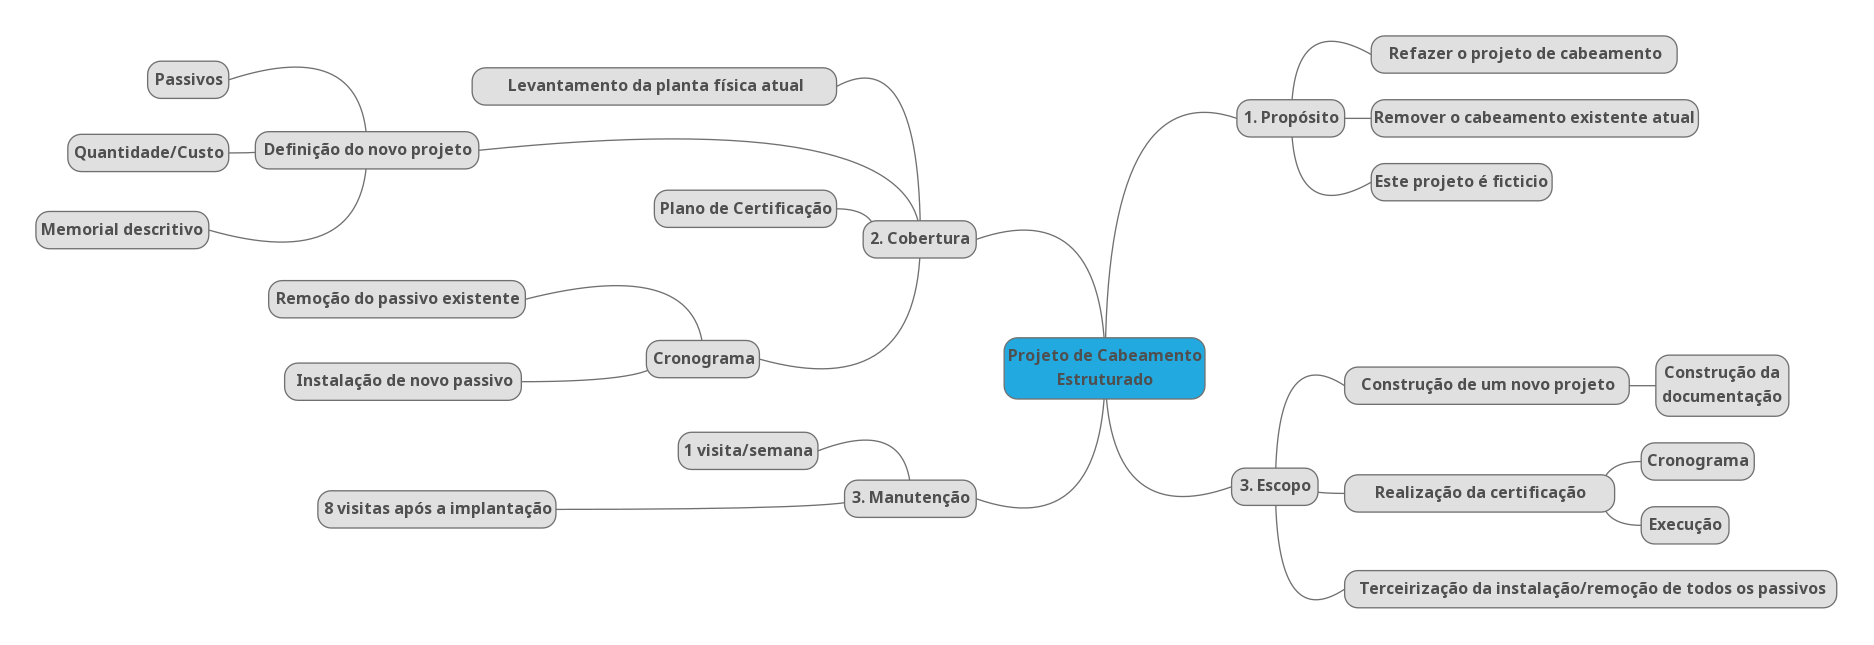
\includegraphics[width=\textwidth,height=5cm,keepaspectratio]{fig4}
%%	\caption{Exemplo de resumo gráfico}
%%	\label{fig6}	
%%\end{figure}

%%\subsubsection{Inserir PDF}

%%Para inserir um arquivo pdf em seu texto utilize o comando includepdf. O arquivo será mapeado no layout corrente.

%%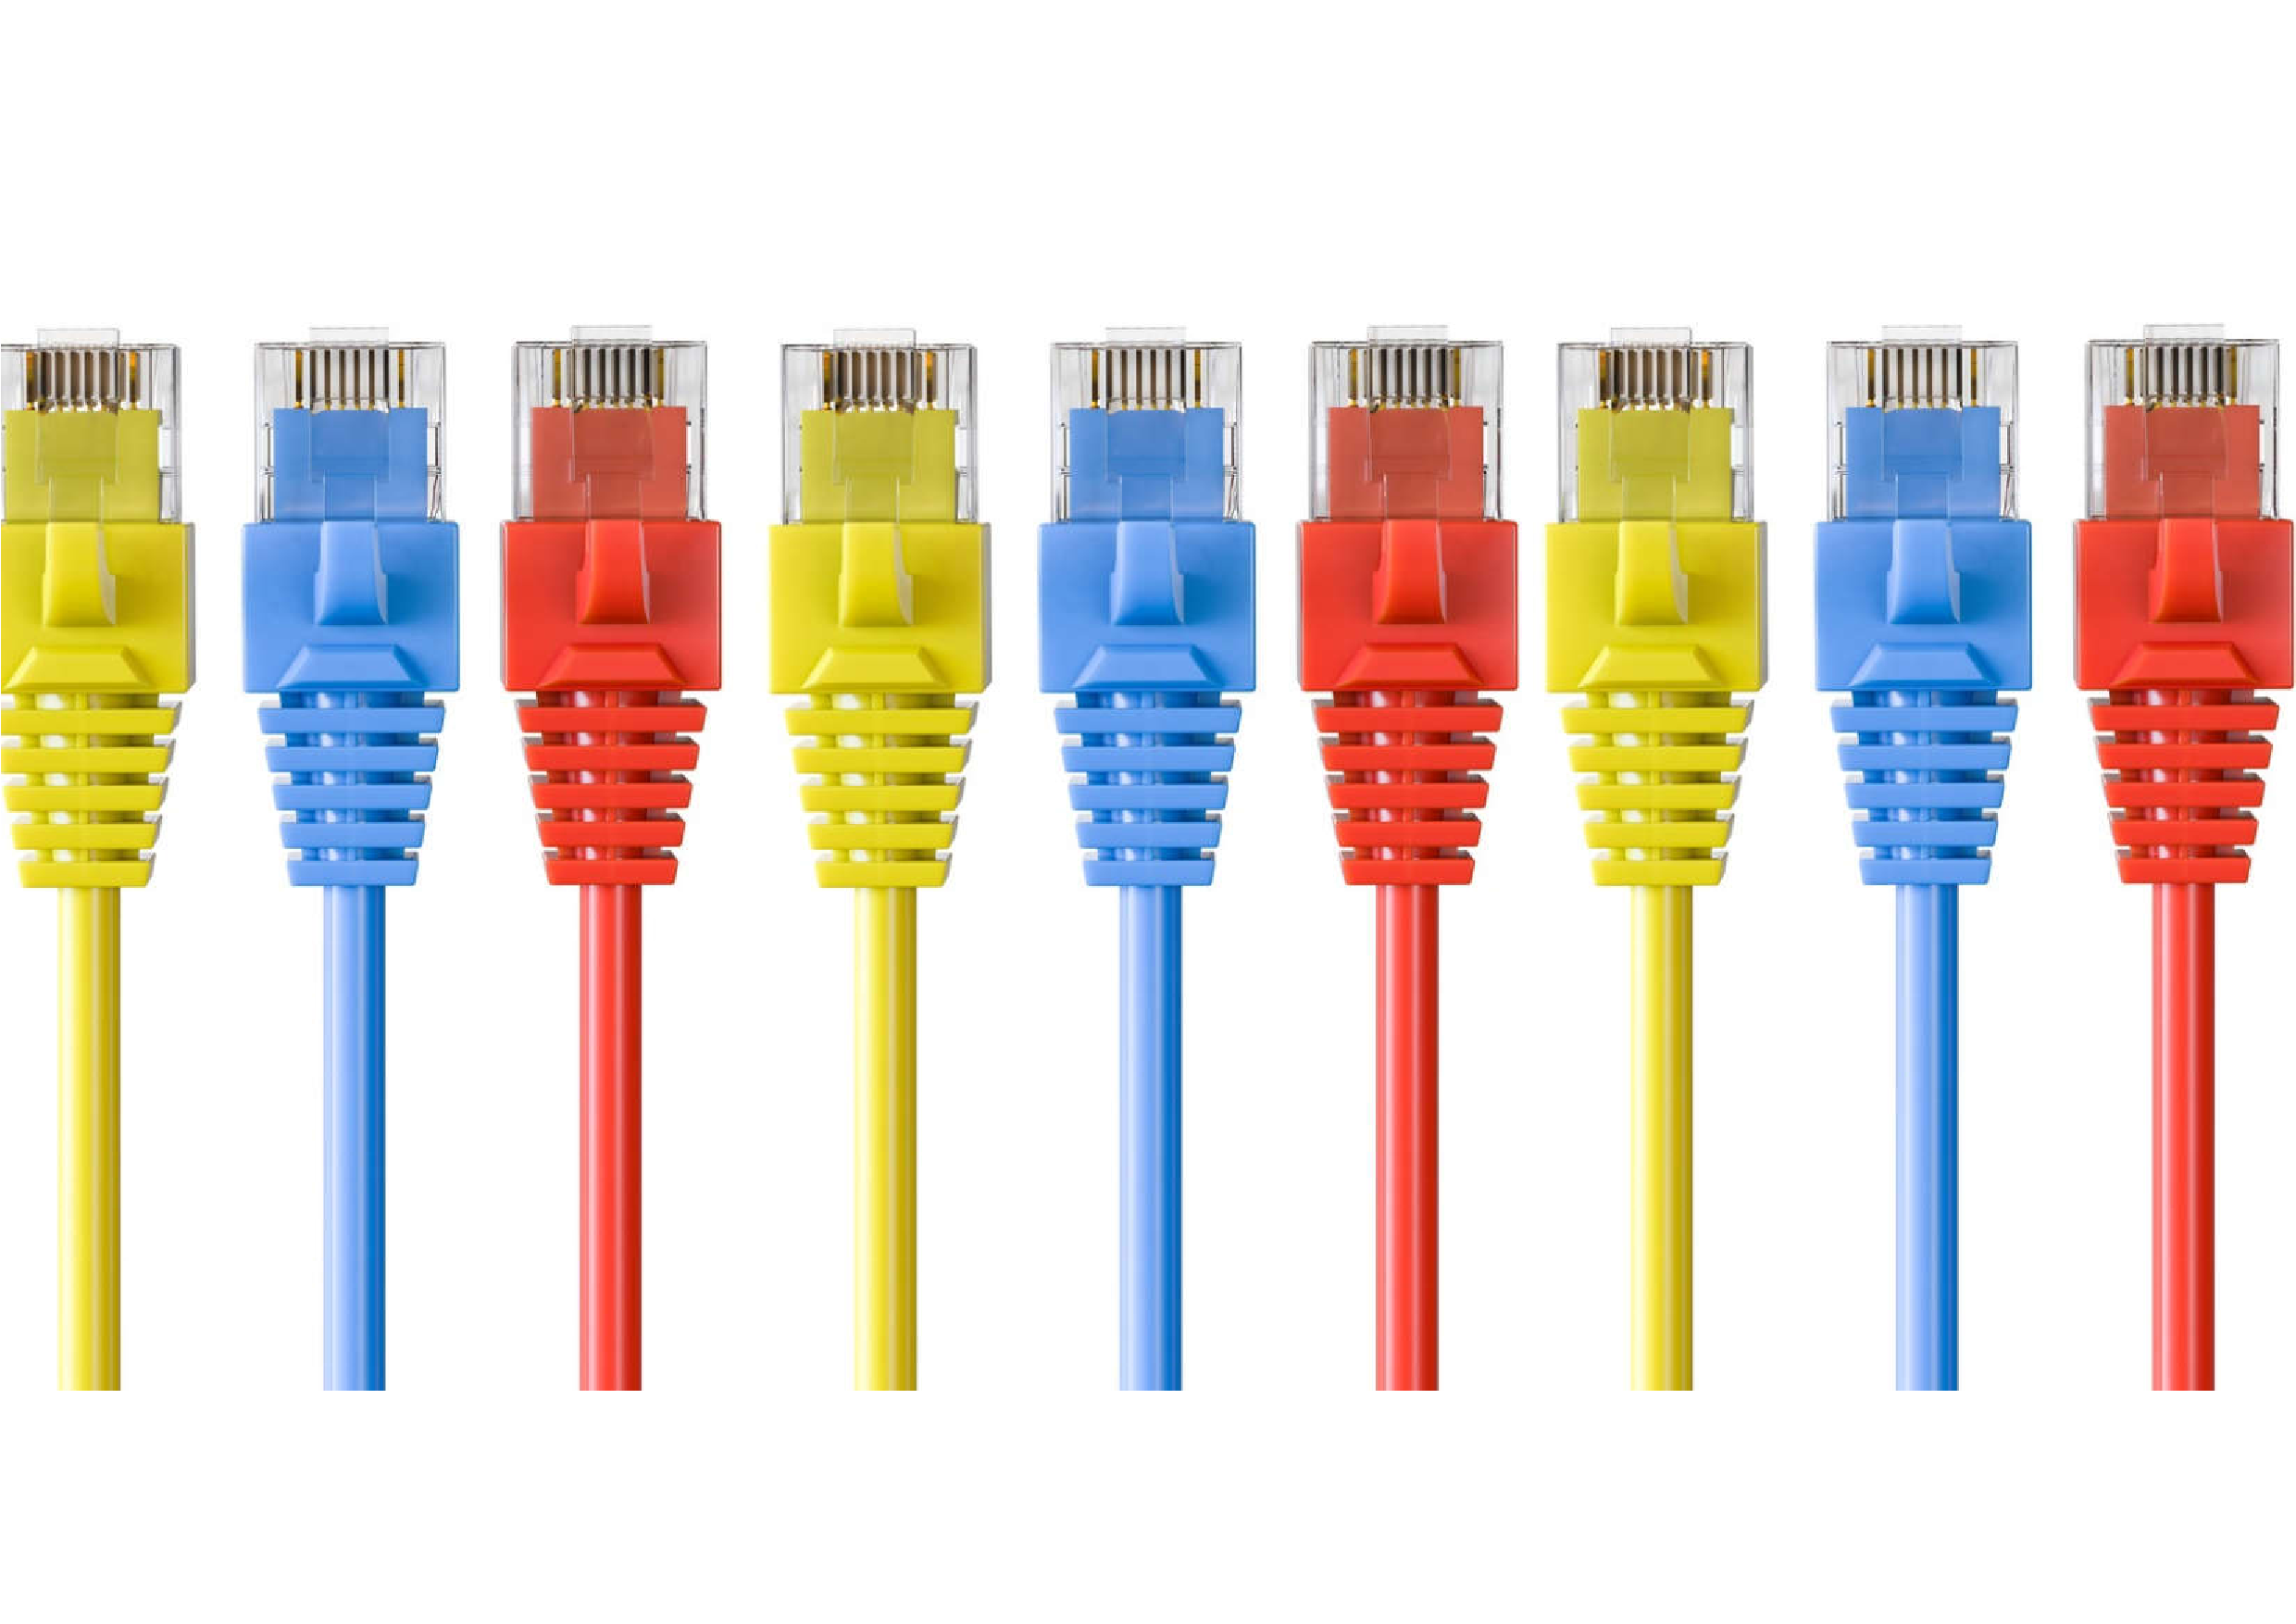
\includepdf{cabling.pdf}
%% ***********************************************************************
%% === ate aqui    =====  ================================================
%% ***********************************************************************

\end{document}